We next evaluate the ability of our entire analysis 
pipeline to identify group differences across temporally evolving \textit{covariance} trajectories. 
In many existing analyses, the effect of the mean differences may be stronger than the effect of the interaction matrix. 
However, in cases where the {\em mean signal is weak}, we expect that the covariance effect will be important. 
To evaluate our model in this regime, we perform a set of simulation studies and also analyze a publicly available longitudinal dataset.

\paragraph{Simulations.} We randomly generate SPD matrices from a `path' of 4 discrete points along the manifold, and use these data 
as population 
covariance matrices to generate 0-mean sample data. Table \ref{tab:recover-table} shows the results of the hypothesis testing 
procedure with 50 features averaged over 100 runs, where both the true number of features with covariance trajectory differences, $p_t$, 
and the number of samples per group, $n$, were varied. 
As expected, our recovery rate increases nicely 
as a function of the number of samples $n$ and decreases as the size of region of change $p_t$ is increased when $n$ is held constant.
	
We compare our model to baseline methods that may be used in practice for the foregoing 
group difference hypothesis test. In standard applications, general linear models (GLMs) are often the first line of attack. 
When the covariates are assumed to be independent, a simple linear model as in \eqref{eq:euclideanhyptest} may be suitable. 
However, when the group difference is influenced by specific interactions between covariates, such linear models require additional care. 
A typical solution is to introduce pairwise interaction terms into the model -- a choice between 
%This requires a critical choice and decision on the user's part: 
all possible interactions or \textit{specific interactions specified by an expert}. The first model has 
%significant 
%risk of overfitting, overwhelmingly so in the case 
problems since the number of samples $n \ll p^2$. In the second model, we depend completely on the user's choice of interactions, 
and must correct for multiple testing when testing different models, at least partly reducing the power of the final test.
%
\begin{figure}
	\begin{center}
		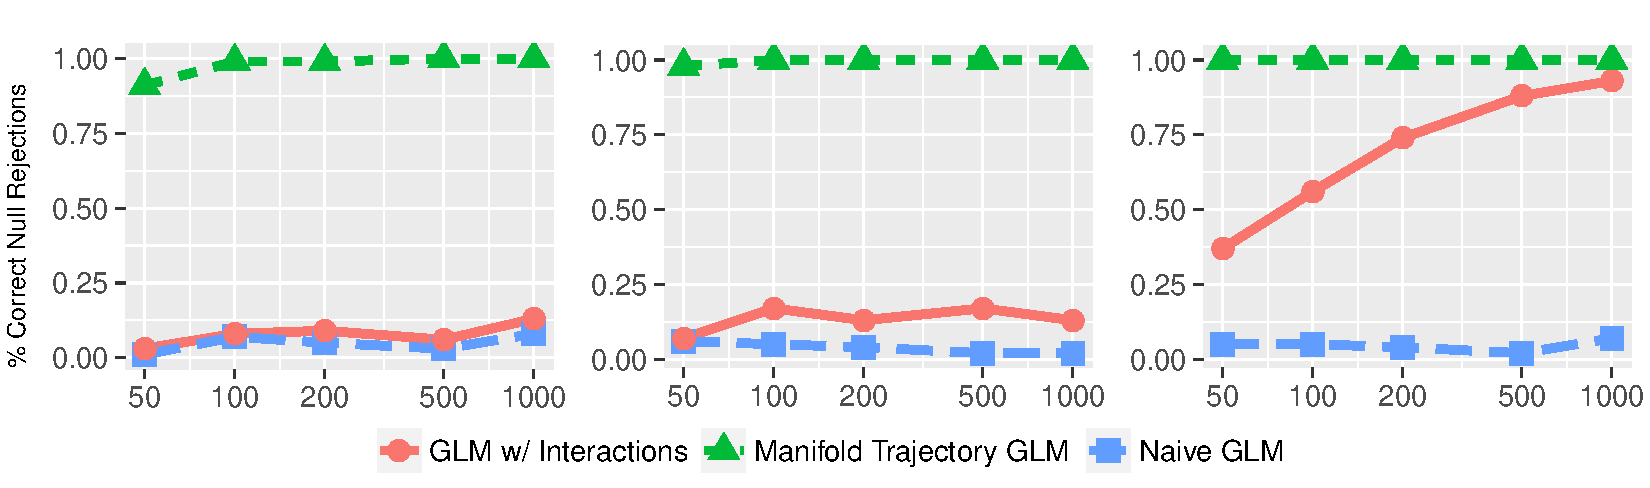
\includegraphics[width=\textwidth]{3_covtraj/figs/sim_results.pdf}
		\caption[Synthetic hypothesis testing true positive rates]{\label{fg:sim_graphs}Correct null hypothesis rejections over 100 runs for three models. For $p = 50$ features, each plot shows the rejection rate
		for $p_t \in \{4, 8, 20\}$ (from left to right) respectively as a function of the number of sample points.}
	\end{center}
\end{figure}
%	
\begin{table}
	{
		\caption{\label{tab:recover-table} Detection Accuracy of hypothesis test scheme (100 runs).}
		\begin{center}
			{\begin{tabular}{lllll}
					\toprule
					\toprule
					& $p_t = 5$& $p_t = 8$	& $p_t = 10$&  $p_t = 15$ 	\\
					\midrule
					$n=10$	&  0.06  &  0.02  &  0.04  &  0.03 \\
					$n=20$	&  0.75  &  0.75  &  0.53  &  0.29 \\
					$n=50$	&  0.99  &  1.00  &  1.00  &  0.80 \\
					$n=100$	&  1.00  &  1.00  &  1.00  &  0.95 \\
					$n=200$	&  1.00  &  1.00  &  1.00  &  0.98 \\
					$n=1000$&  1.00  &  1.00  &  1.00  &  1.00 \\
					\bottomrule
					\bottomrule
			\end{tabular}}
		\end{center}
	}
\end{table}
\todo{ch3: check table style in more recent chapters}
Figure \ref{fg:sim_graphs} shows the value of our method over these models. For the interaction GLM case, we randomly select interaction terms to include in the GLM, with size $p_t$ (the ground truth number of variables in the interaction). In this way, we approximate the effect of an oracle specifying to the GLM which terms may describe the underlying interaction. 
We report the fraction of significance tests where a significance threshold 
of $p \leq 0.05$ was found for each model, averaged over 100 runs. 
%Simulated data were generated using the procedure outlined for the simulations above, with more details provided in the Appendix.
We see that our proposed scheme consistently achieves near-perfect results in terms of the percentage of null hypotheses that 
were correctly rejected (i.e., there was a significant group-difference signal). The power of scan statistics on 
graphs is particularly evident in the needle in haystack setting where the true differential signal is small ($p_t \leq 8$)
and the sample size is small to medium. When the sample size is large and $p_t$ is also large, the standard linear model with additional interaction terms starts to approach the statistical performance of our algorithm.

%% \begin{figure}[]
%% 	\begin{center}
%% 		\includegraphics[width=0.9\textwidth]{babynames_result_bad.pdf}
%% 		\caption{\label{fig:babyEX} Baby name orderings over time across boys and girls.}
%% 	\end{center}
%% \end{figure}
